\documentclass[a4paper]{report}
\author{Jure Kos}
\title{Vaja 49, Prehodni pojavi v električnih krogih}
\date{3.3.2022}
\usepackage{graphicx}
\graphicspath{ {./images/} }

\begin{document}
\maketitle


\chapter*{Uvod}
Vaja obravnava prehodne pojave v vezju upornika-R, kondenzatorja-C in induktorja-L, kot so: 
\subsection{Praznjenje kondenzatorja:}
 \graphicspath{ {./Images/} }
\[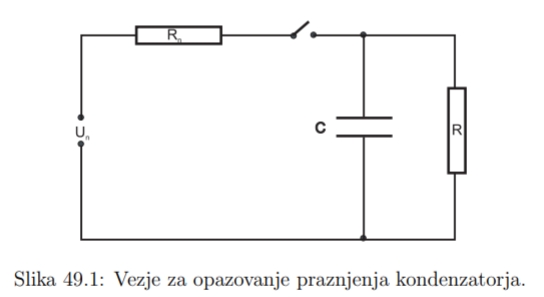
\includegraphics[scale=0.95]{49 slika 1.png}\]\\
Naj bo stikalo na začetku sklenjeno. Na kondenzatorju bo potem napetost enaka $U_0=\frac{U_n}{R+R_n}$, tok na uporniku pa $I_0=\frac{U_0}{R}$.\\
Ko prekinemo zveze z izvirom napetosti , začne naboj odtekati s pozitivne plošče kondenzatorja na negativno ploščo. Posledično se napetost med ploščama zmanjšuje.\\
Napetost-U na kondenzatorju poganja tok $I = \frac{U}{R}$ tako, da se naboj zmanjšuje:
\[I = \frac{-de}{dt} = \frac{CdU}{dt}.\]
Ko izenačimo oba izraza za tok, dobimo diferencialno enačbo: 
\[\frac{dU}{dt} + \frac{1}{RC}U = 0\]\\
katera določa časovno spreminjanje napetosti na kondenzatorju. Rešitev enačbe pa je: 
\[U = U_0e^{-t/\tau}\]
Rešitev prikazuje, da napetost eksponentno pojema z relaksacijskim časom-$\tau = RC$. To je čas, v katerem se napetost na kondenzatorju e-krat pomanjša. Namesto relaksacijskega časa radi podamo tudi razpolovni čas $t^{1/2}$ (čas, v katerem se napetost zmanjša na polovico začetne).\\
Velja:
\[t^{1/2} = \tau ln 2 = 0,693 \cdot RC\]

\section*{Polnjenje kondenzatorja:}

\[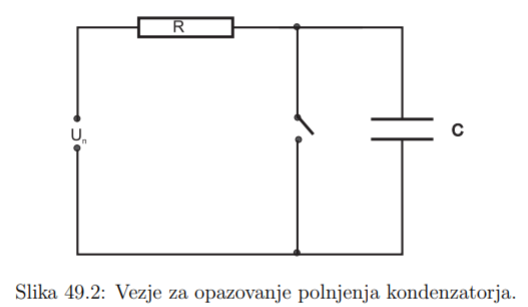
\includegraphics[scale=0.95]{49 slika 2.png}\]

Naj bo na začetku stikalo sklenjeno, na kondenzatorju pa napetost enaka 0. Ko stikalo razklenemo, električni tok-I steče v kondenzator in ga začne polniti. V vsakem trenutku velja: \[U_n = U + IR.\]
Kjer je U-napetost na kondenzatorju. Tok polni kondenzator, zato velja: \[I = \frac{de}{dt} = \frac{Cdu}{dt}.\]
Ta izraz vstavimo v prvo enačbo in po preureditvi dobimo diferencialno enačbo: 
\[\frac{dU}{dt} + \left(\frac{1}{RC}\right)U = \frac{U_n}{RC}\]
Ob času t = 0 je na kondenzatorju napetost 0, zato je rešitev enačbe:
\[U = U_n \left(1-e^{-t/\tau}\right)\]
Napetost na kondenzatorju se eksponentno približuje končni vrednosti $U_n$.

\section*{Dušeno nihanje nihajnega kroga:}

\[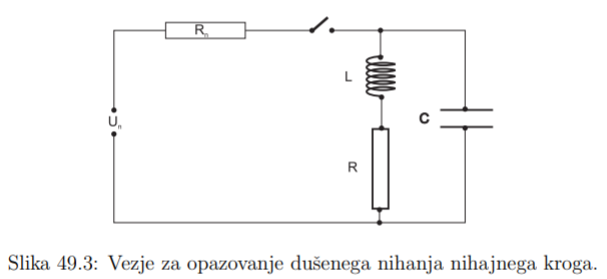
\includegraphics[scale=0.95]{49 slika 3.png}\]
Naj bo v danem trenutku napetost na kondenzatorju U, po krogih pa teče tok I. Vsota napetosti tuljave in kondenzatorja mora biti enaka 0:
\[ U-L \frac{dI}{dt}-RI=0\]
Kjer je $\frac{-LdI}{dt}$ napetost zaradi induktivnosti in (-RI) napetost na uporu tuljave.\\
Naboj na kondenzatorju črpa tok $I=\frac{-de}{dt} = \frac{-CdU}{dt}$. 
Če vstavimo izraza tako dobimo difrencialno enačbo:
\[\frac{d^2U}{dt^2}+2\frac{\beta dU}{dt}+\omega{_0^2}U = 0\]
Kjer je $2\beta = \frac{R}{L}$, $\omega{_0^2} = \frac{1}{LC},\beta$-koeficient dušenja in $\omega_0$-lastna frekvenca nedušenega kroga\\
Posledično velja:
\[U = e^{-\beta t} \left(A sin \omega t + B cos \omega t \right)\]
\[\omega = \sqrt{\left(\omega{_0^2}- \beta^2 \right)}\]

Koeficienta A in B sta ob času t = 0 odvisna od začetnih pogojev (začetne napetosti in od začetnega toka). Pri našem poizkusu je do časa t = 0 krog priklopljen na izvir napetosti. Skozi tuljavo ob t = 0 teče enosmerni tok $I=\frac{U_n}{R+R_n}$, napetost na kondenzatorju pa je $U_0=I_0R$. Ko vir napetosti ob času t = 0 odklopimo, za kratek hip ostanejo razmere v krogu še nespremenjene, le da takrat tok $I_0$  teče zaradi naboja na kondenzatorju. Računsko bi začetne pogoje zato zapisali kot: 
\[U_0 = I_0R\] 
\[\left(\frac{dU}{dt} \right)_0 =\frac{-I_0}{C}\]
\[I_0 = \left(-\frac{de}{dt} \right)_0 = -C \left(\frac{dU}{dt} \right)_0\]
Z vstavitvijo tega pogoja v začetni izraz, dobimo enačbi za koeficienta A in B:\\
\[A= I_0R \left(\frac{\beta}{\omega}- \frac{1}{\omega RC} \right)\]
\[B=I_0R\]
Odvisnost napetosti od časa računsko torej zapišemo kot:

Glede na dane podatke: $R = 200\Omega$, $L = 1,227 H, C = 0,25 \mu F$ je člen $\frac{1}{\omega RC}$ veliko večji od drugih, zato velja $\omega = \omega_0$ in tako velja enačba:
\[U = -\left(\frac{I_0}{\omega_0 C}\right)e^{-\beta t}sin\omega_0t\]

\chapter*{Naloga}
1. Opazuj z osciloskopom polnjenje in praznjenje kondenzatorja. Izmeri in izračunaj relaksacijski čas iz znanih podatkov in primerjaj obe vrednosti. Časovni potek napetosti na kondenzatorju nariši na milimetrski papir.\\
\\
2. Z osciloskopom opazuj dušeno nihanje nihajnega kroga. Izmeri in izračunaj frekvenco kroga, koeficient dušenja in začetni tok po krogu.\\
\\
\section*{Potrebščine}
1. Osciloskop,\\
2. periodično stikalo, \\
3. stikalna plošča, \\
4. upori, kondenzatorji ter tuljava na vtičnih podložkah in\\
5. usmernik.
\newpage


\chapter*{Meritve}
\section*{Praznenje kondenzatorja}
$$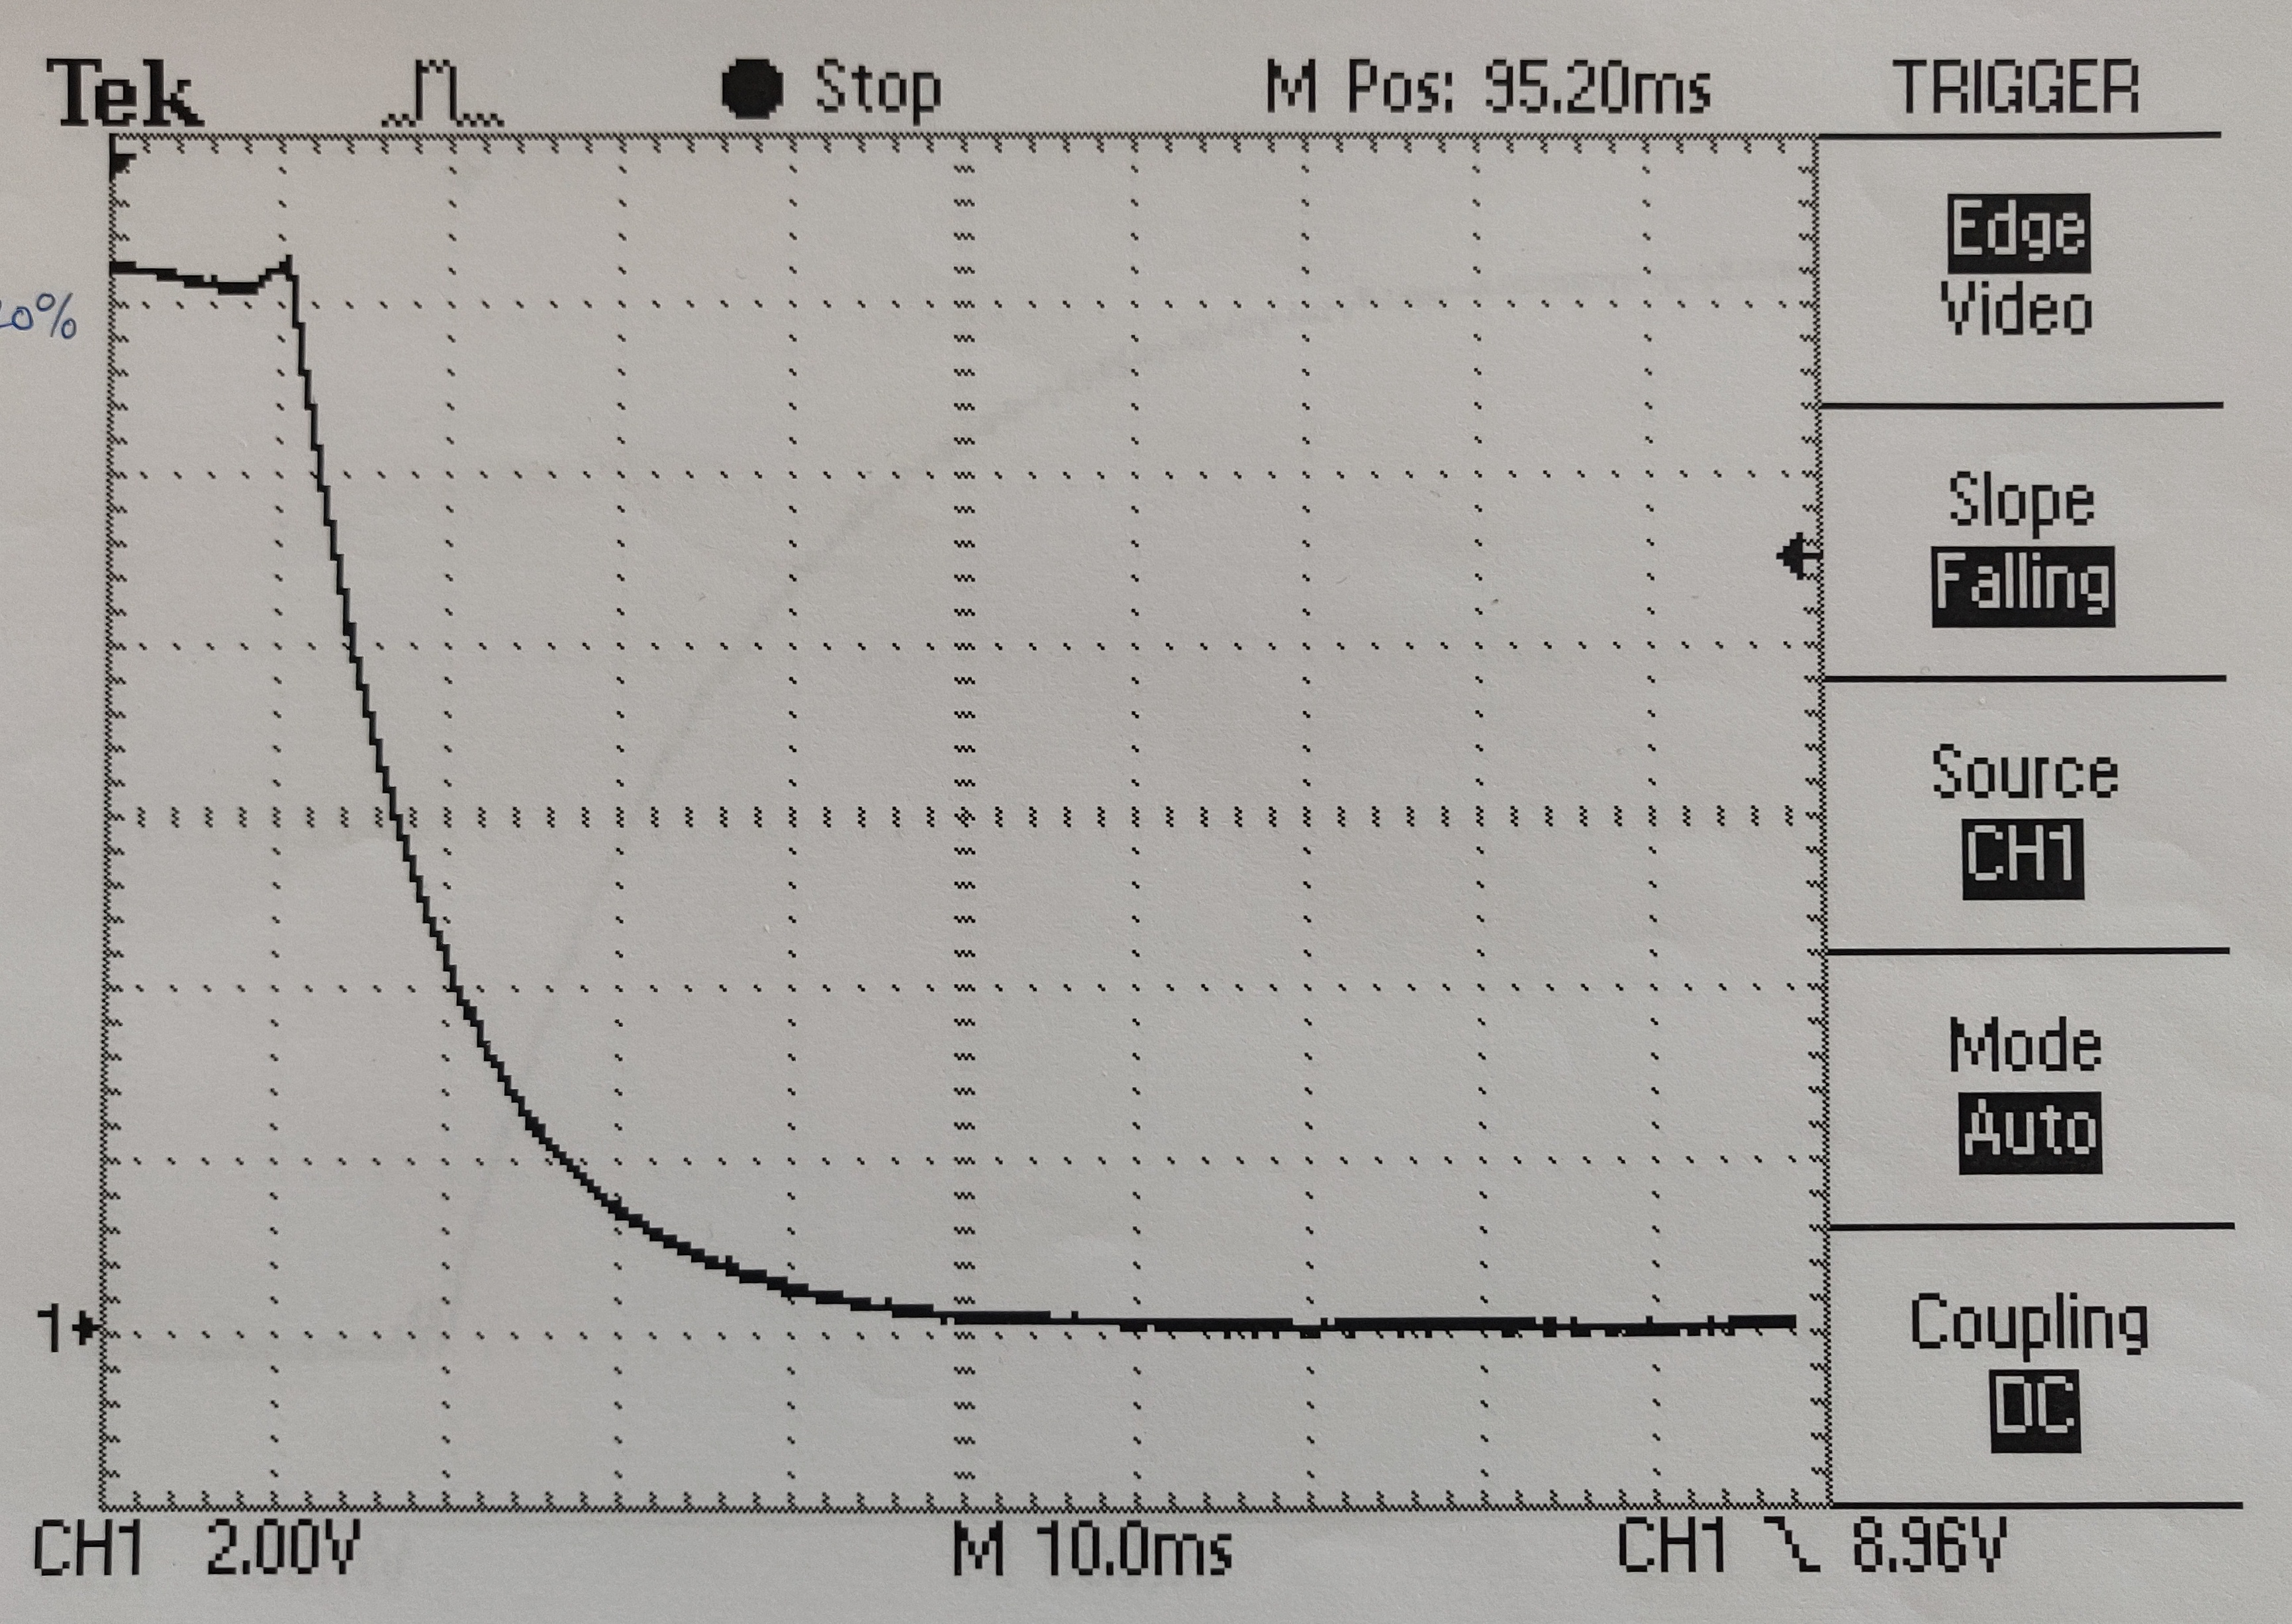
\includegraphics[width=\textwidth]{Praznenje.png}$$
\begin{table}[h!]
  \begin{center}
    \label{tab:table1}
    \begin{tabular}{|c|c|c|} 
    \hline
      Št. točke & t [ms] & U [V]\\
      \hline
      1 & 0 & 3,15\\
      2 & 5 & 1,95\\
      3 & 10 & 1,10\\
      4 & 15 & 0,60\\
      5 & 20 & 0,35\\
      6 & 25 & 0,20\\
      7 & 30 & 0,15\\
      8 & 35 & 0,05\\
      \hline
    \end{tabular}
  \end{center}
\end{table}
\[R = 3,8  k\Omega \hspace{5mm} C = 0,25 \mu F\] 
\[U_0 = 3,15 V\]
\section*{Polnjenje kondenzatorja}
$$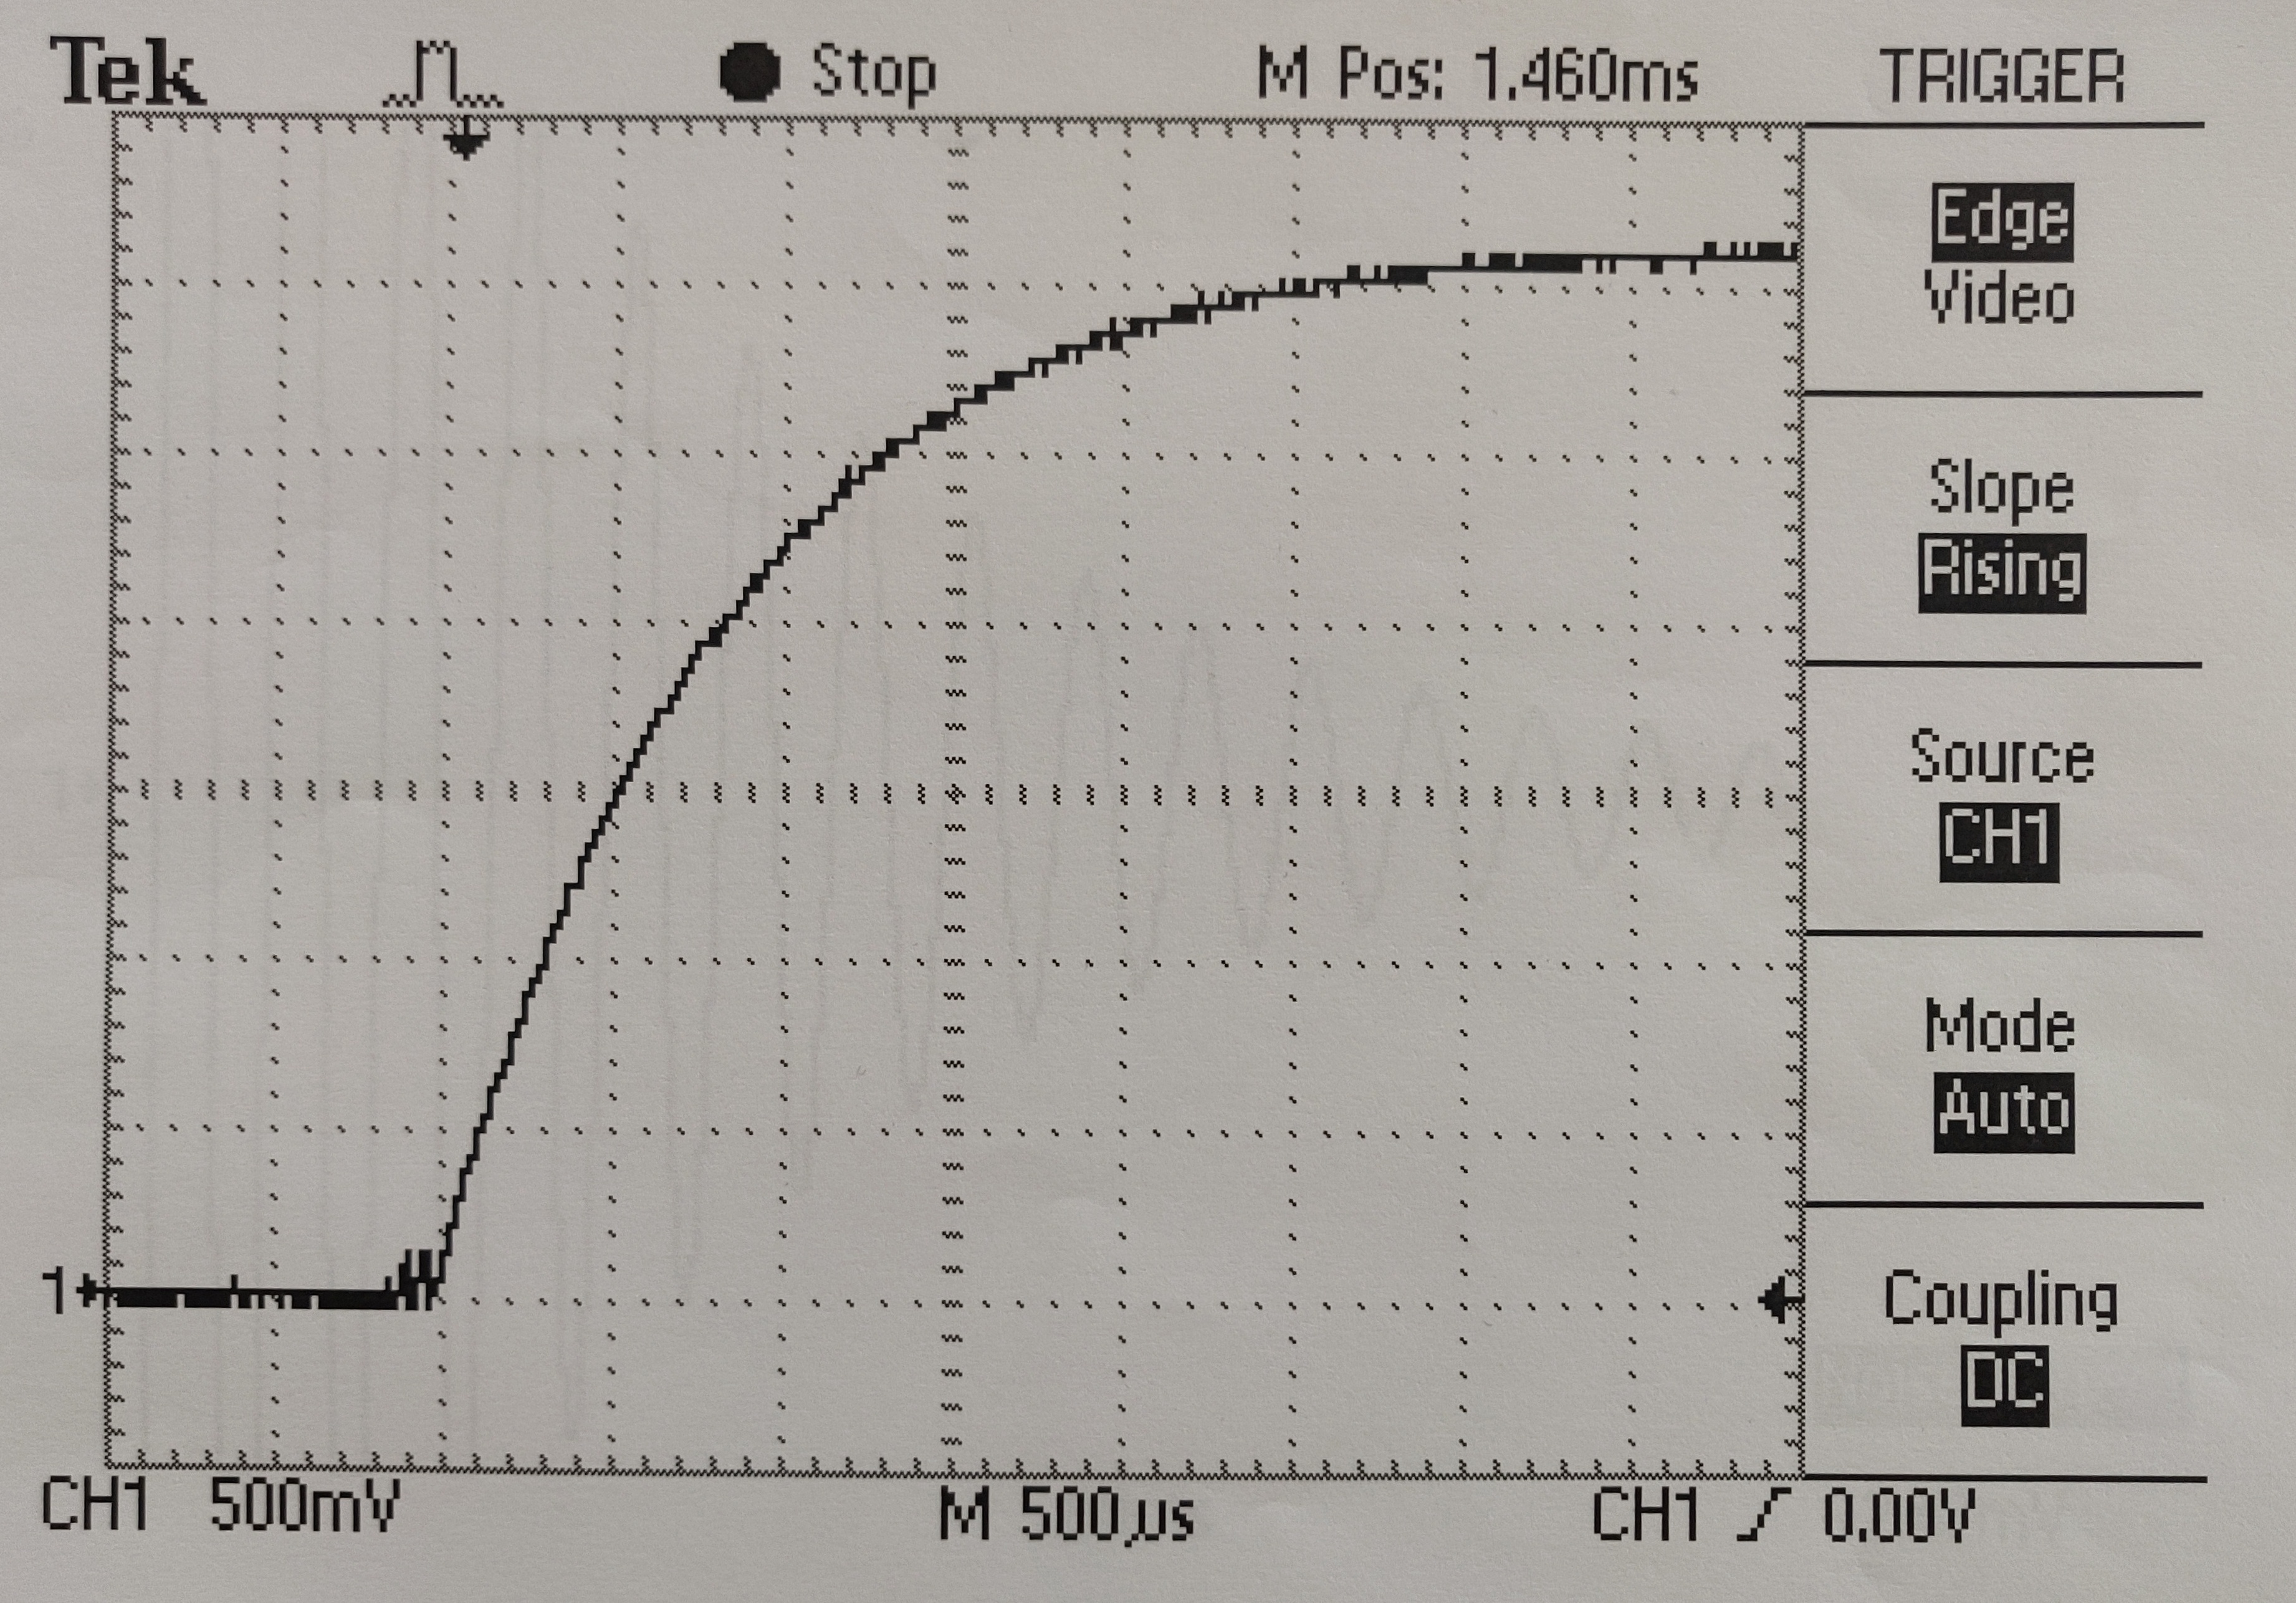
\includegraphics[width=\textwidth]{Polnjenje.png}$$
\begin{table}[h!]
  \begin{center}
    \label{tab:table1}
    \begin{tabular}{|c|c|c|}
     \hline
      Št. točke & t [ms] & U [V]\\
      \hline
      1 & 0,0 & 0,00\\
      2 & 0,5 & 1,50\\
      3 & 1,0 & 2,20\\
      4 & 1,5 & 2,35\\
      5 & 2,0 & 2,80\\
      6 & 2,5 & 3,00\\
      7 & 3,0 & 3,05\\
      8 & 3,5 & 3,10\\
      \hline
    \end{tabular}
  \end{center}
\end{table}
\[R = 27 M \Omega \hspace{5mm}  C = 1000 pF\]  
\[U_0 = 3,1 V\]

\section*{Dušeno nihanje}
$$\includegraphics[width=\textwidth]{Dušenje.png}$$
\begin{table}[h!]
  \begin{center}
    \label{tab:table1}
    \begin{tabular}{|c|c|c|} 
    \hline
      Št. točke & t [ms] &U [V]\\
      \hline
      1 & 4 & -1,95\\
      2 & 7 & -1,50\\
      3 & 11 & -1,20\\
      4 & 14 & -0,95\\
      5 & 17 & -0,75\\
      6 & 21 & -0,60\\
      7 & 24 & -0,45\\
      8 & 27 & -0,40\\
      \hline
    \end{tabular}
  \end{center}
\end{table}
\[ R = 138 \Omega, C = 0,25  \mu F \hspace{5mm} L = 1,227H\]
\[U_0 = 2,20  V\]
\chapter*{Računi}

\section*{Praznenje kondenzatora}
V grafu ln(U/$U_0$) v odvisnosti od časa je naklon (k) enak $\frac{-1}{\tau _i}$. Za primerjavo pa lahko izračunamo še po enačbi: $\tau_r = RC$\\
$$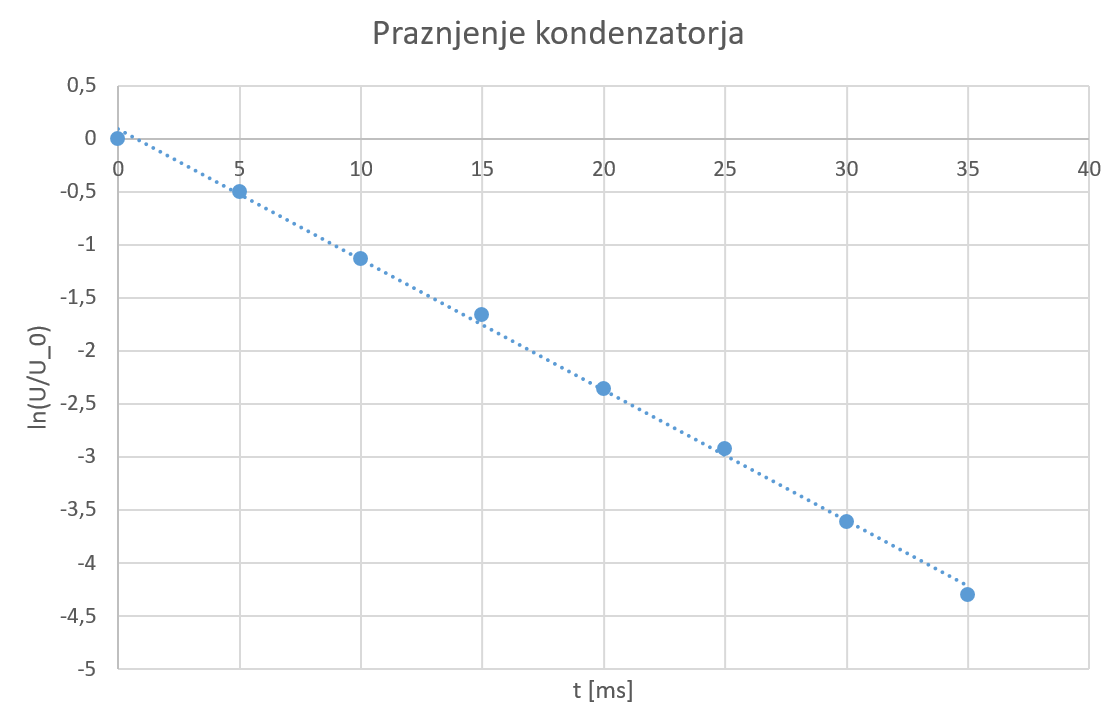
\includegraphics[scale=0.45]{49 - Praznjenje kondenzatorja.png}$$\\

\[k = -0,123 \cdot 10^{-3}  s^{-1}\cdot (1 \pm 0,01) \Rightarrow \tau_i = 8,10 \cdot 10^{-3}s  (1 \pm 0,01)\] 

\[\tau_r = 9,4 \cdot 10^{-3}s \cdot (1 \pm 0,07)\]

\section*{Polnjenje kondenzatorja}
V grafu ln(1 - U/$U_0$) v odvisnosti od časa-t je naklon-k enak $1/\tau_i$.
$$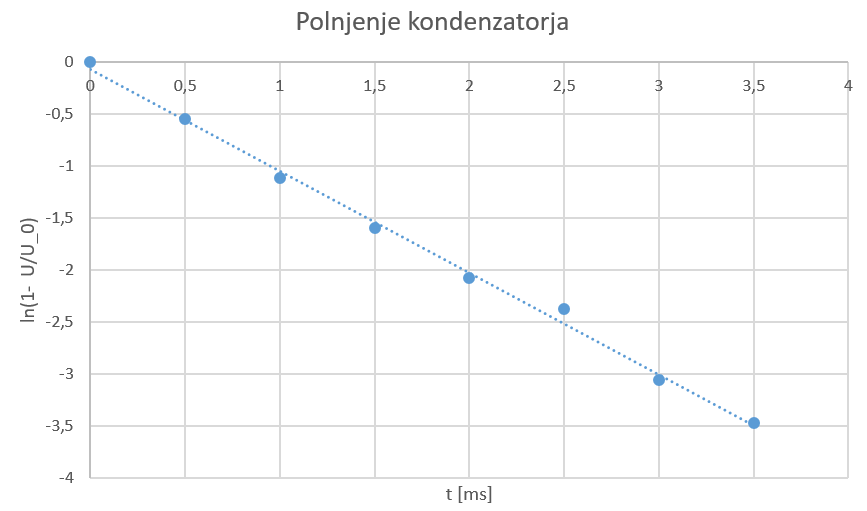
\includegraphics[scale=0.55]{49 - Polnjenje kondenzatorja.png}$$\\

\[k = -0,98 \cdot 10^{-3} s^{-1} \cdot (1 \pm 0,01) \Rightarrow\]

\[\tau_i = 1,02 \cdot 10^{-3} s \cdot (1 \pm 0,01)\]


\section*{Dušeno nihanje}
Nihajni čas 

\[t_0 = 3 ms \Rightarrow \omega_0 = 2\pi/t_0 = 2,1 ms^{-1}\]

\noindent Krožno frekvenco lahko še izračunamo po enačbi:

\[\omega_0 = \sqrt{1/LC} = 1,81  ms^{-1}\]

\noindent Iz zaporednih amplitud se da določiti koeficient dušenja $-\beta$, saj velja: $ln(U_1/U_2) = \beta(t_2 - t_1)$. Posledično velja:

\[\beta = \frac{ln(U_1/U_2)}{(t_2 - t_1)} = \frac{R}{2L} = 56 s^{-1}\]

\noindent Začetni tok $I_0$ pa izračunamo po enačbi:

\[I_0 = \frac{U_0}{R} = 16  mA\pm 1mA\]
\end{document}
